\documentclass[bachelor, och, coursework]{SCWorks}
% параметр - тип обучения - одно из значений:
%    spec     - специальность
%    bachelor - бакалавриат (по умолчанию)
%    master   - магистратура
% параметр - форма обучения - одно из значений:
%    och   - очное (по умолчанию)
%    zaoch - заочное
% параметр - тип работы - одно из значений:
%    referat    - реферат
%    coursework - курсовая работа (по умолчанию)
%    diploma    - дипломная работа
%    pract      - отчет по практике
% параметр - включение шрифта
%    times    - включение шрифта Times New Roman (если установлен)
%               по умолчанию выключен
\usepackage{subfigure}
\usepackage{tikz,pgfplots}
\pgfplotsset{compat=1.5}
\usepackage{float}

%\usepackage{titlesec}
\setcounter{secnumdepth}{4}
%\titleformat{\paragraph}
%{\normalfont\normalsize}{\theparagraph}{1em}{}
%\titlespacing*{\paragraph}
%{35.5pt}{3.25ex plus 1ex minus .2ex}{1.5ex plus .2ex}

\titleformat{\paragraph}[block]
{\hspace{1.25cm}\normalfont}
{\theparagraph}{1ex}{}
\titlespacing{\paragraph}
{0cm}{2ex plus 1ex minus .2ex}{.4ex plus.2ex}

% --------------------------------------------------------------------------%


\usepackage[T2A]{fontenc}
\usepackage[utf8]{inputenc}
\usepackage{graphicx}
\graphicspath{ {./images/} }
\usepackage{tempora}

\usepackage[sort,compress]{cite}
\usepackage{amsmath}
\usepackage{amssymb}
\usepackage{amsthm}
\usepackage{fancyvrb}
\usepackage{listings}
\usepackage{listingsutf8}
\usepackage{longtable}
\usepackage{array}
\usepackage[english,russian]{babel}

% \usepackage[colorlinks=true]{hyperref}
\usepackage{url}

\usepackage{underscore}
\usepackage{setspace}
\usepackage{indentfirst} 
\usepackage{mathtools}
\usepackage{amsfonts}
\usepackage{enumitem}
\usepackage{tikz}
\usepackage{minted}

\newcommand{\eqdef}{\stackrel {\rm def}{=}}
\newcommand{\specialcell}[2][c]{%
\begin{tabular}[#1]{@{}c@{}}#2\end{tabular}}

\renewcommand\theFancyVerbLine{\small\arabic{FancyVerbLine}}

\newtheorem{lem}{Лемма}

\begin{document}

% Кафедра (в родительном падеже)
\chair{теоретических основ компьютерной безопасности и криптографии}

% Тема работы
\title{Обнаружение сетевого RDP трафика методом анализа его поведения}

% Курс
\course{3}

% Группа
\group{331}

% Факультет (в родительном падеже) (по умолчанию "факультета КНиИТ")
\department{факультета КНиИТ}

% Специальность/направление код - наименование
%\napravlenie{09.03.04 "--- Программная инженерия}
%\napravlenie{010500 "--- Математическое обеспечение и администрирование информационных систем}
%\napravlenie{230100 "--- Информатика и вычислительная техника}
%\napravlenie{231000 "--- Программная инженерия}
\napravlenie{10.05.01 "--- Компьютерная безопасность}

% Для студентки. Для работы студента следующая команда не нужна.
% \studenttitle{Студентки}

% Фамилия, имя, отчество в родительном падеже
\author{Токарева Никиты Сергеевича}

% Заведующий кафедрой
\chtitle{} % степень, звание
\chname{Абросимов М. Б.}

%Научный руководитель (для реферата преподаватель проверяющий работу)
\satitle{доцент} %должность, степень, звание
\saname{Гортинский А. В.}

% Руководитель практики от организации (только для практики,
% для остальных типов работ не используется)
% \patitle{к.ф.-м.н.}
% \paname{С.~В.~Миронов}

% Семестр (только для практики, для остальных
% типов работ не используется)
%\term{8}

% Наименование практики (только для практики, для остальных
% типов работ не используется)
%\practtype{преддипломная}

% Продолжительность практики (количество недель) (только для практики,
% для остальных типов работ не используется)
%\duration{4}

% Даты начала и окончания практики (только для практики, для остальных
% типов работ не используется)
%\practStart{30.04.2019}
%\practFinish{27.05.2019}

% Год выполнения отчета
\date{2022}

\maketitle

% Включение нумерации рисунков, формул и таблиц по разделам
% (по умолчанию - нумерация сквозная)
% (допускается оба вида нумерации)
% \secNumbering

%-------------------------------------------------------------------------------------------

\tableofcontents

\intro
Информация -- это сведения об окружающем мире и протекающих в нём процессах, которые зафиксированы на каком-либо носителе.
Благодаря протоколам удаленного доступа можно распоряжаться базами данных, информацией, которая хранится на другом устройстве. В недавнем прошлом большинство
схем удаленного доступа характеризовалось высокой стоимостью, низкой производительностью, небольшой скоростью передачи данных, недостаточным уровнем защищенности
передаваемой информации \cite{1}. 

Сейчас, когда практически все предприятия перешли на дистанционный формат работы, компании выбирают протокол RDP, так как он прост в настройке и в использовании.
Но далеко не все уделяют особое внимание безопасности собственных рабочих мест. Поэтому предприятия могут быть атакованы злоумышленниками.

В данной работе будут разобраны принцип работы RDP, анализ его поведения, а также методы обнаружения данного протокола.

\section{Определение RDP}

Протокол RDP (от англ. Remote Desktop Protocol --- протокол удалённого рабочего стола) --- патентованный протокол 
прикладного уровня компании Microsoft и приобретен ею у другой компании Polycom, который предоставляет пользователю графический интерфейс для 
подключения к другому компьютеру через сетевое соединение. Для этого пользователь запускает клиентское программное обеспечение RDP, а на другом 
компьютере должно быть запущено программное обеспечение сервера RDP \cite{2}.

Клиенты для подключения по RDP существуют для большинства версий Microsoft Windows, Linux, Unix, macOS, iOS, Android и 
других операционных систем. Стоит отметить, что RDP-серверы встроены в операционные системы Windows. По умолчанию подключения, созданные с 
помощью RDP, используют UDP-порт 3389 и TCP порт 3389, по которым осуществляется передача данных.

\subsection{Безопасность протокола RDP}

Как уже известно, что для операционной системы Windows постоянно выходят различные обновления, включая обновлений RDS (от англ. Remote Desktop Services --- службы 
удаленных рабочих столов). В связи с этим возникают различные уязвимости при инициализации RDP-сессии. В основном они не связаны непосредственно с
протоколом RDP, но касаются службы удаленных рабочих столов RDS и позволяют при успешной эксплуатации путем отправления специального запроса через RDP
получить возможность выполнения произвольного кода на уязвимой системе, даже не проходя при этом процедуру проверки подлинности. Достаточно лишь иметь доступ
к хосту или серверу с уязвимой системой Windows. Таким образом, любая система, доступная из сети Интернет, является уязвимой при отсутствии установленных
последних обновлений безопасности Windows.

Если стоит задача защитить удаленный доступ, то, конечно, необходимо использовать надежный пароль, обновить свое программное обеспечение до последней версии,
также можно использовать VPN подключение, чтобы получить IP-адрес виртуальной сети и добавить его в правило исключения брандмауэра RDP. Стоит отметить, что
существует много разных способов, чтобы защитить подключение с помощью протокола RDP и более подробно это описано в документации Microsoft.

  \section{Принцип работы протокола RDP и анализ его поведения}

  Принцип работы RDP базируется на протоколе TCP. Соединение клиент-сервер происходит на транспортном уровне. После инициализации пользователь 
  проходит аутентификацию. В случае успешного подтверждения сервер передает клиенту управление. Стоит отметить, что под понятием слова <<клиент>> подразумевается
  любое устройство (персональный компьютер, планшет или смартфон), а <<сервер>> --- удаленный компьютер, к которому оно подключается.

  Протокол RDP внутри себя поддерживает виртуальные каналы, через которые пользователю передаются дополнительные функции операционной системы,
  например, можно распечатать документ, воспроизвести видео или скопировать файл в буфер обмена.

  % Известно, что RDP является прикладным протоколом, базирующимся на TCP. Для начала пользователю необходимо установить соединение клиент-сервер, которое
  % происходит на транспортном уровне. После инициализации RDP-сессии производится аутентификация. Далее сервер начинает передавать клиенту графический вывод и
  % ожидает входные данные от клавиатуры и мыши. В качестве графического вывода может выступать как точная копия графического экрана, передаваемая как изображение,
  % так и команды на отрисовку графических примитивов, например, линия, круг, эллипс, текст и др. Для протокола RDP приоритетом является передача вывода с помощью
  % примитивов, так как это экономит трафик. Изображение передается только в том случае, если не удалось согласовать параметры передачи примитивов при установке 
  % RDP-сессии. Обработка полученных команд и вывод изображения осуществляется с помощью графической подсистемы RDP-клинта. Сигнал нажатия и отпускания клавиши клавиатуры
  % шифруются и ожидают команды отправки \cite{3}.
  
  Далее в работе будет описан процесс установки RDP-сессии, во время которой осуществляется захват трафика с помощью одной известной программы Wireshark. С помощью нее
  можно достаточно подробно рассмотреть структуру сообщений протоколов.

  Для начала будет произведено подключение с помощью <<Удаленного рабочего стола>>. Это средство представляет собой встроенную в Windows программу, предназначенную
  для удалённого доступа. При его использовании предполагается, что пользователь будет подключаться к одному компьютеру с другого устройства, находящегося в той же
  локальной сети. В качестве клиента и сервера будут выступать компьютеры с операционной системой Windows 10 Professional версии 21H2. 
  
  % Стоит отметить, что
  % программа <<Удаленный рабочий стол>> может работать только в том случае, если клиент имеет операционную систему Windows, macOS, Android и iOS и 
  % сервер может находится на платформах Windows, сделанных только в редакциях Professional, Enterprise и Ultimate. Поэтому, пользуясь данной программой, 
  % не к каждой платформе можно будет подключится.
  
  Для подключения к удаленному рабочему столу были заданы статические IP-адреса. Клиенту был присвоен статический IP-адрес 192.168.10.254,
  а серверу --- 192.168.10.229, соответственно маска сети 255.255.255.0. После того, как были заданы IP-адреса, необходимо зайти в настройки
  Windows, чтобы включить возможность подключения к удаленному рабочему столу. Об этом более подробно описано
  в статьях \cite{userdp1} и \cite{userdp2}. Далее на сервере был произведен запуск анализа трафика с помощью приложения Wireshark.
  После подключения к удаленному компьютеру программа-анализатор трафика начала <<захватывать>> пакеты, как показано на рисунке \ref{wireshark1},
  принадлежащие следующим протоколам:
  
  \begin{figure}[H]
    \centering
    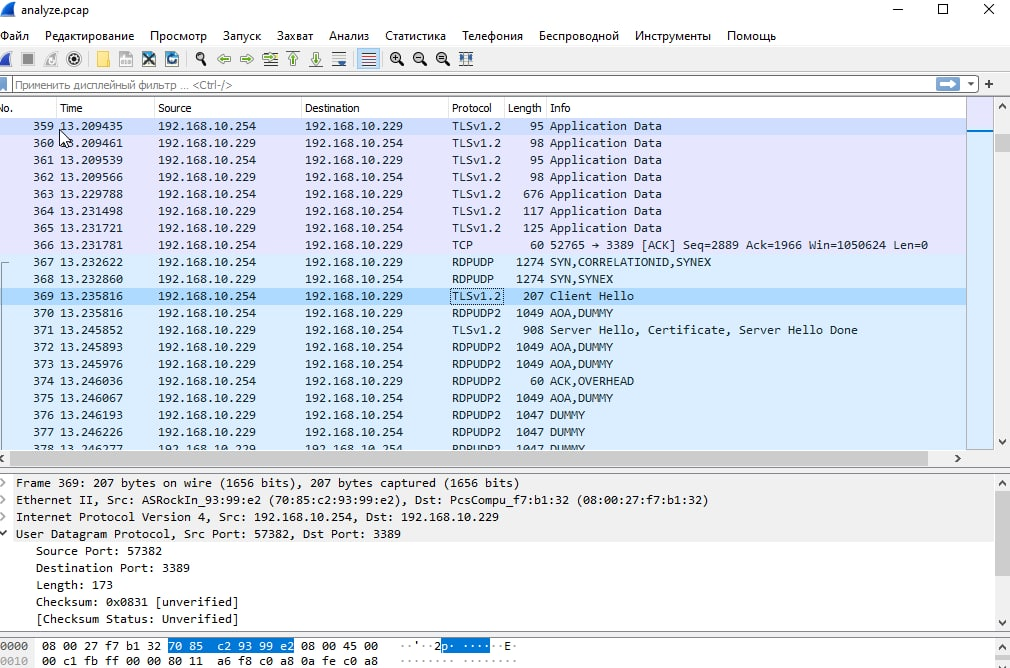
\includegraphics[width=0.8\textwidth]{photo/wireshark1.png}
    \caption{Окно программы Wireshark после захвата трафика}
    \label{wireshark1}
  \end{figure}

  \begin{itemize}
    \item RDPUDP --- протокол RDP, использующий для передачи данных UDP-протокол.
    \item RDPUDP2 также относится к протоколу RDP. Он был разработан для повышения производительности сетевого соединения по сравнению
    с соответствующим соединением RDP-UDP \cite{rdpudp}. 
    \item TLSv1.2 --- протокол защиты транспортного уровня, обеспечивающий защищенную передачу между узлами в сети интернет. В данном случае обеспечивает
    безопасность RDP-сессии.
  \end{itemize}
  
  Во время работы программы Wireshark было найдено достаточное количество пакетов, принадлежащих RDP, которые содержат в себе достаточно интересную
  информацию. Поэтому стоит рассказать о том, как происходит стандартный способ защиты RDP. Это можно представить в несколько этапов:

  \begin{enumerate}
    \item Клиент объявляет серверу о своем намерении использовать стандартный протокол RDP.
    \item Сервер соглашается с этим и отправляет клиенту свой собственный открытый ключ, полученный при шифровании алгоритмом RSA, а также некоторую строку
    случайных байтов (обычно её называют <<random сервером>>), генерируемую сервером. На рисунке \ref{rndserv} можно увидеть запись random сервера.

    \begin{figure}[H]
      \centering
      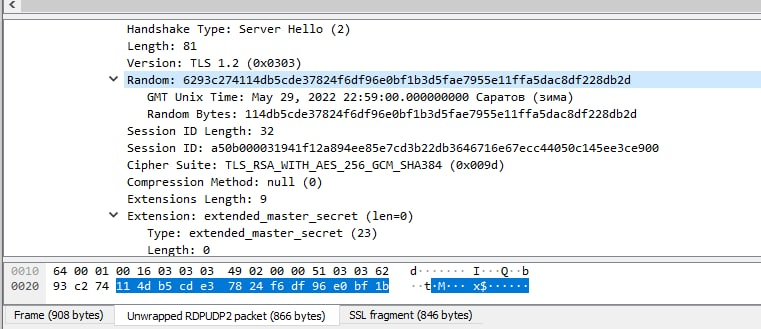
\includegraphics[width=0.9\textwidth]{photo/rndserv.png}
      \caption{Содержимое пакета, посылаемого от сервера клиенту (запись random сервера)}
      \label{rndserv}
    \end{figure}

    Совокупность открытого ключа и некоторая строка случайных байтов называется <<сертификатом>>. Данная запись изображена на рисунке \ref{cert}.
    
    \begin{figure}[H]
      \centering
      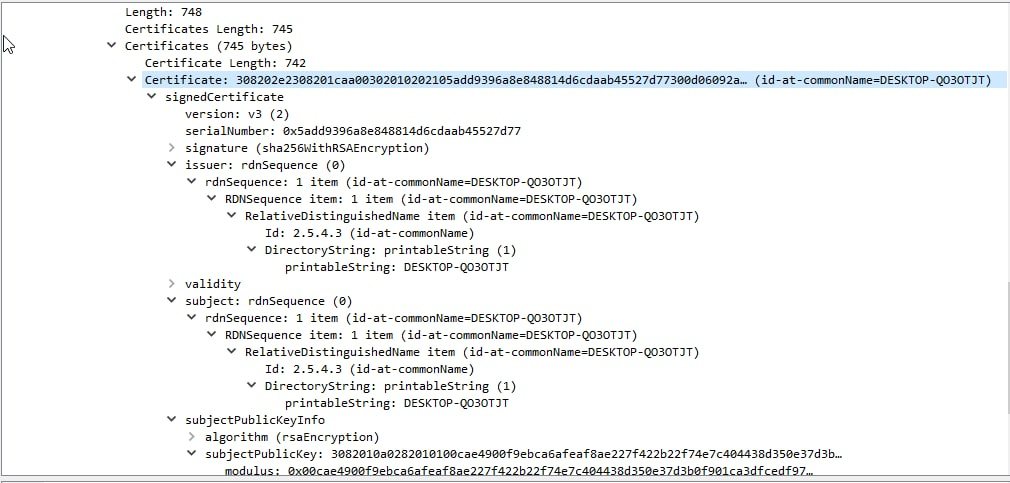
\includegraphics[width=0.9\textwidth]{photo/cert.png}
      \caption{Содержимое пакета, посылаемого от сервера клиенту (запись сертификата)}
      \label{cert}
    \end{figure}
    
    Сертификат подписывается службой терминалов, например, RDS, с использованием закрытого ключа для обеспечения подлинности.

    \item Теперь клиент посылает некоторую строку случайных байтов, которая называется <<premaster secret>>, показанная на рисунке \ref{cert1}. 
    
    \begin{figure}[H]
      \centering
      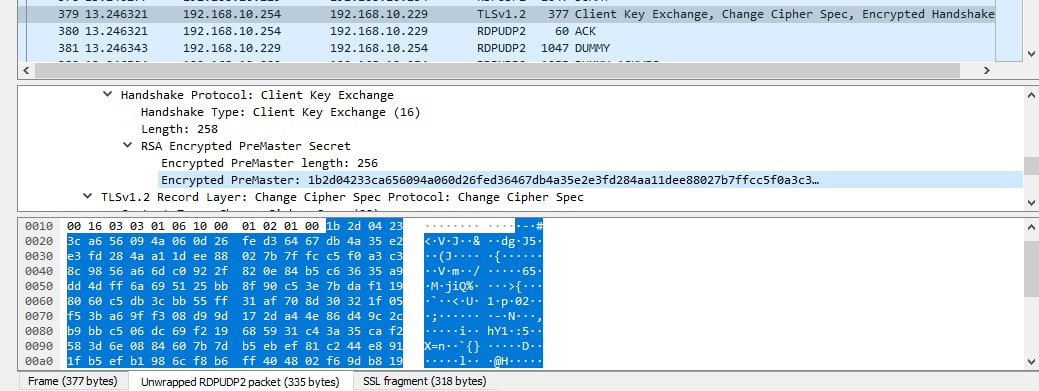
\includegraphics[width=0.9\textwidth]{photo/cert1.png}
      \caption{Содержимое пакета, посылаемого от клиента серверу (запись premaster secret)}
      \label{cert1}
    \end{figure}
    
    Данная запись шифруется открытым ключом, которая может быть расшифрована сервером только с помощью закрытого ключа службы терминалов.
    \item Сервер расшифровывает premaster secret с помощью собственного закрытого ключа.
    \item В случае успеха клиент и сервер получают свои сеансовые ключи из random сервера и premaster secret. Далее они используются для симметричного 
    шифрования остальной части сеанса.
  \end{enumerate}

  После того как был произведен разбор RDP-сессии в некоторых пакетах можно заметить сообщения, принадлежащие протоколу TLS.
  На рисунке \ref{clnt-hello} видно, что в раскодированной последовательности чисел имеется IP-адрес сервера.

  \begin{figure}[H]
    \centering
    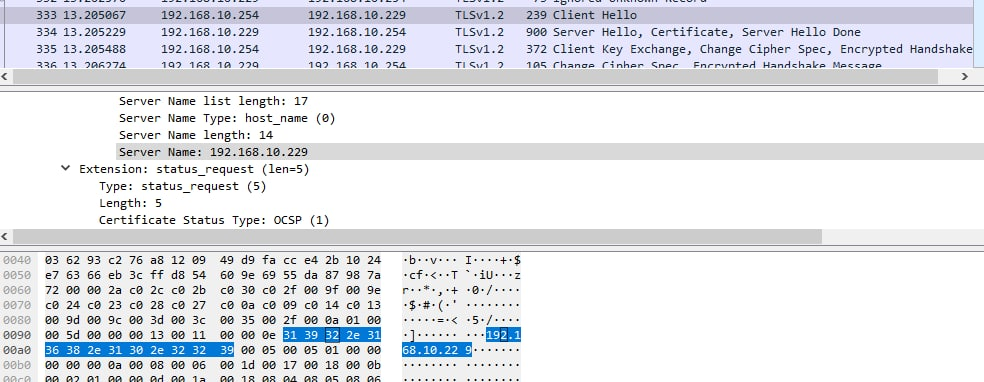
\includegraphics[width=0.9\textwidth]{photo/clnt-hello.jpg}
    \caption{Данные пакета, посылаемого клиентом}
    \label{clnt-hello}
  \end{figure}  

  А следующим за ним идет пакет, в котором можно заметить имя сервера, как показано на рисунке \ref{serv-hello}.

  \begin{figure}[H]
    \centering
    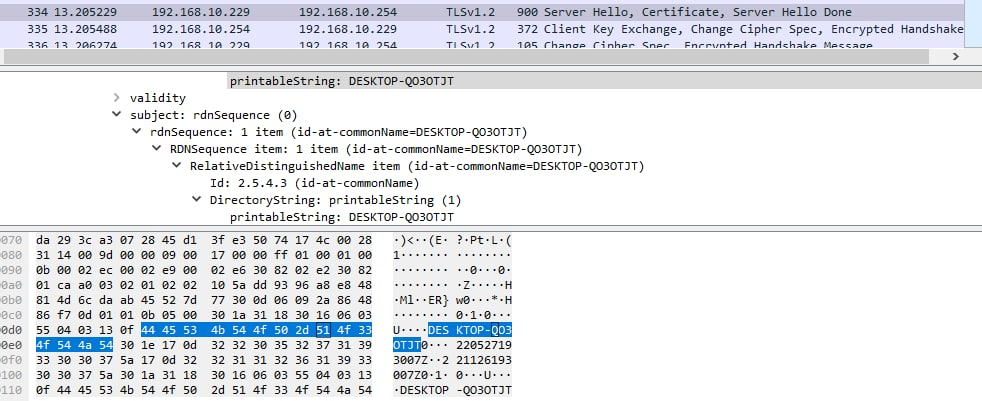
\includegraphics[width=0.9\textwidth]{photo/serv-hello.jpg}
    \caption{Данные пакета, посылаемого сервером}
    \label{serv-hello}
  \end{figure}

  Такие пакеты были перехвачены в момент установки RDP-сессии, в то время, когда клиент успешно ввел пароль и его сертификат
  был одобрен сервером. Т.е. по данным сообщениям можно понять, что к устройству с IP-адресом 192.168.10.229 было совершено
  подключение через 3389-й порт. Значит в этот момент времени начиналась установка RDP-сессии.
  
  Осталось понять, как обнаружить подключение к удаленному рабочему столу по протоколу RDP.

  % \section{Обнаружение сеанса удаленного управления}

  % Помимо программы <<Удаленный рабочий стол>> есть и другие приложения, с помощью которых можно установить соединение клиент-сервер. Например:
  
  % \begin{enumerate}
  %   \item Удаленный рабочий стол Chrome (Chrome Remote Desktop) --- удаленный рабочий стол Chrome позволяет пользователям получать удаленный
  %   доступ к другому компьютеру через браузер Chrome. С помощью данного приложения можно подключаться к платформам, на которых есть этот браузер.
  %   Однако подключение таким образом к телефону невозможно, так как мобильное приложение «Удалённый рабочий стол Chrome» предоставляет доступ к компьютеру.
  %   \item TeamViewer --- приложение, позволяющее установить соединение с любым персональным компьютером или сервером всего за несколько секунд. На данный
  %   момент это очень популярное приложение, которое позволяет записывать сеансы на видео, общаться участникам в голосовом и текстовом каналах и открывать
  %   удалённый доступ только к выбранным приложениям.
  %   \item Remote Utilities --- программа для удалённого подключения к компьютерам. Серверная часть Remote Utilities устанавливается только на Windows,
  %   зато клиенты доступны на всех популярных платформах.
  %   \item Ammyy Admin --- надежный и удобный инструмент для удаленного доступа к компьютеру. Программа позволяет удалённо перезагружать компьютер,
  %   входить в систему и менять пользователей. Однако она доступна только для Windows.
  % \end{enumerate}

  % Сейчас таких программ, позволяющих подключиться к удаленному рабочему столу, стало достаточно много. И в некоторых приложениях уже не используется RDP.
  % Например, программа Chrome Remote Desktop работает с протоколом HTTP, а TeamViewer вообще использует собственный проприетарный протокол, который не
  % задокументирован. Хотя он немного похож на RDP по назначению, но включает в себя обход преобразования сетевых адресов и имеет немного другие методы аутентификации.
  % Поэтому некоторые программы, созданные для распознавания и перехвата RDP трафика, в данном случае будут бесполезны.

  % Хорошо, что такие программы, позволяющие устанавливать соединение с рабочим столом, для пользователя имеются в открытом доступе. Что, если существуют такие приложения,
  % о которых пользователь не имеет никакого представления? Получается, данное программное обеспечение будет являться потенциальной угрозой, так как
  % с помощью него можно подключиться к удаленному рабочему столу без разрешения самого пользователя.
  
  % Таким образом, в данной ситуации необходимо проанализировать возможную угрозу, используя различные методы обнаружения RDP-сессии.
    
  \section{Обнаружение сеанса удаленного управления с помощью программы}
  
  Одним из методов выявления сообщений, передаваемых по сети, является сниффер --- это программное обеспечение, которое анализирует входящий и исходящий трафик с компьютера, подключенного к
  интернету. Для данной работы была написана на языке Python программа, перехватывающая трафик сети, которая также может обнаружить подключение по
  протоколу RDP.
    
  Данный сниффер принимает пакеты четвертой версии интернет-протоко- \\* ла, пакеты IPv4, содержащие в поле данных сообщения протоколов других уровней. В
  этом случае здесь будут рассматриваться сообщения протоколов транспортного уровня, в частности TCP и UDP.
    
  При запуске программы появится запрос на выбор <<прослушиваемого>> порта. По умолчанию будет задан RDP-порт 3389. Далее, для того чтобы успешно
  перехватить пакет, необходимо установить неразборчивый режим на сетевой интерфейс, чтобы сетевая плата принимала все пакеты независимо от того,
  кому они адресованы. Данный выбор
  зависит от способа подключения устройства к сети. Например, в Linux есть виртуальный интерфейс (<<lo>>), который ваш компьютер использует для связи с
  самим собой, также существуют интерфейсы относящиеся к проводному соединению (<<enp0s3>>) и беспроводному (<<wlp2s0>>). В данном случае все устройства
  будут подключены к сети через Ethernet. Затем программа должна обратиться к файлу <<white-list.log>>, в котором содержится информация об устройствах,
  находящиеся в одной локальной сети. Допустим в файл не был записан один компьютер, тогда в случае создания подключения по RDP-протоколу программа посчитает его
  неизвестным и запишет в файл <<information.log>>, в котором будет содержаться вся информация о посторонних попытках создания RDP-сессии.

    Функция get\_white\_list() формирует пары: имя и IP-адрес компьютера. К каждой такой паре сопоставляется пара записи имени и IP-адреса устройства в
    шестнадцатеричной системе счисления. Этот список нужен для анализа данных, хранящихся в TCP-сегменте.

    \begin{minted}[fontsize=\footnotesize]{Python}
      # Получение списка верифицированных устройств
      def get_white_list():
        f = open('white-list.log', 'r')
        while True:
          line = f.readline().replace('\n', '')
          if '#' in line:
            continue
          if not line:
            break
          pos = line.find('::')
          serv_name = line[:pos]
          serv_ip = line[pos + 2:]
          white_list[(serv_name, serv_ip)] = (convert_string(serv_name), convert_string(serv_ip))

      # Форматирование строки в hex-код
      def convert_string(string):
        s = ''
        for el in bytearray(string.encode('utf-8')):
          s += '\\' + str(hex(el))[1:]
        return s
    \end{minted}

    Функция write\_to\_file() выполняет роль записи в файл <<information.log>> сообщений в зависимости от случая подключения по протоколу RDP. 
    При демонстрации работы программы будет видно, какая информация в нем находится.
    
    \begin{minted}[fontsize=\footnotesize]{Python}
      # Запись в файл
      def write_to_file(tup, bl):
        try:
          time = str(datetime.datetime.now()).split('.')[0]
          with open('information.log', 'a+') as f:
            if bl:
              f.write('Было совершено подключение: ' + time)
              f.write( '\nIP адрес неизвестного клиента: ' + str(tup[0]) + 
                       ' MAC-адрес: ' + tup[1] )
              f.write( '\nПодключение к ПК ' + tup[2] + ' от порта ' + str(tup[3]) + 
                       ' к ' + str(tup[4]) + '\n' )
            else:
              f.write('Время попытки подключения: ' + time)
              f.write( '\nIP адрес неизвестного клиента: ' + str(tup[0]) + 
                       ' MAC-адрес: ' + tup[1] )
              f.write( '\nПодключение осуществлялось к ПК ' + tup[2] + ' от порта ' + 
                       str(tup[3]) + ' к ' + str(tup[4]) + '\n' )
            f.close()
        except:
          pass
    \end{minted}

    Для анализа трафика в сети был создан сокет --- программный интерфейс для обеспечения обмена данными между процессами. В силу заданных параметров он
    получал пакеты, представленные в виде некоторой последовательности чисел, записанных в шестнадцатеричной системе счисления.
    
    \begin{minted}[fontsize=\footnotesize]{Python}
      server = socket.socket(socket.AF_PACKET, socket.SOCK_RAW, socket.ntohs(3))
    \end{minted}
    
    Чтобы раскодировать данную последовательность чисел, необходимо обратиться к структуре пакета. Для начала нужно рассмотреть кадр Ethernet, представленный
    на рисунке \ref{eth-frame}.
    
    \begin{figure}[H]
      \centering
      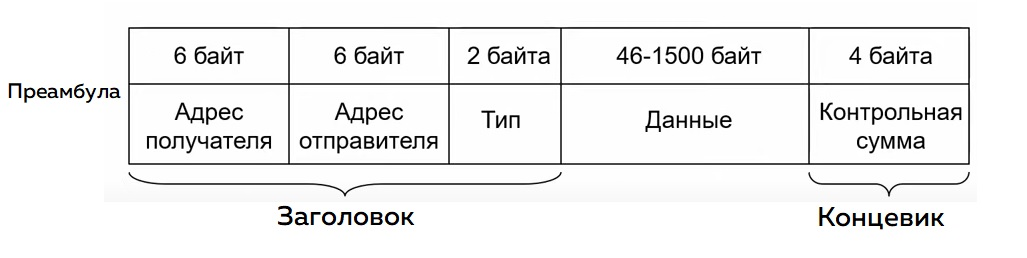
\includegraphics[width=0.9\textwidth]{photo/eth-frame.jpg}
      \caption{Структура Ethernet кадра}
      \label{eth-frame}
    \end{figure}
    
    Стоит отметить, что в данном заголовке нужно раскодировать 14 байт, 12 из которых MAC-адреса получателя и отправителя и 2 байта, идентифицирующие протокол
    сетевого уровня. К примеру 0x0800 -- Ipv4, 0x86DD -- IPv6 и т.д. С помощью функций get\_ethernet\_frame() и get\_mac\_addr() производится получение всех необходимых
    данных заголовка Ethernet.
    
    \begin{minted}[fontsize=\footnotesize]{Python}
      # Получение ethernet-кадра
      def get_ethernet_frame(data):
        dest_mac, src_mac, proto = struct.unpack('!6s6sH', data[:14])
        return get_mac_addr(dest_mac), get_mac_addr(src_mac), socket.htons(proto)
      
      
      # Получение MAC-адреса
        def get_mac_addr(mac_bytes):
          mac_str = ''
          for el in mac_bytes:
            mac_str += format(el, '02x').upper() + ':'
          return mac_str[:len(mac_str) - 1]
      \end{minted}

    После получения информации об Ethernet кадре идет раскодирование интернет-протокола. В данной работе будут рассматриваться пакеты протокола IPv4, 
    так как для обнаружения RDP-сессии этого вполне достаточно. Поэтому необходимо рассмотреть IPv4-заголовок, который показан на рисунке \ref{ipv4-header}.

    \begin{figure}[H]
      \centering
      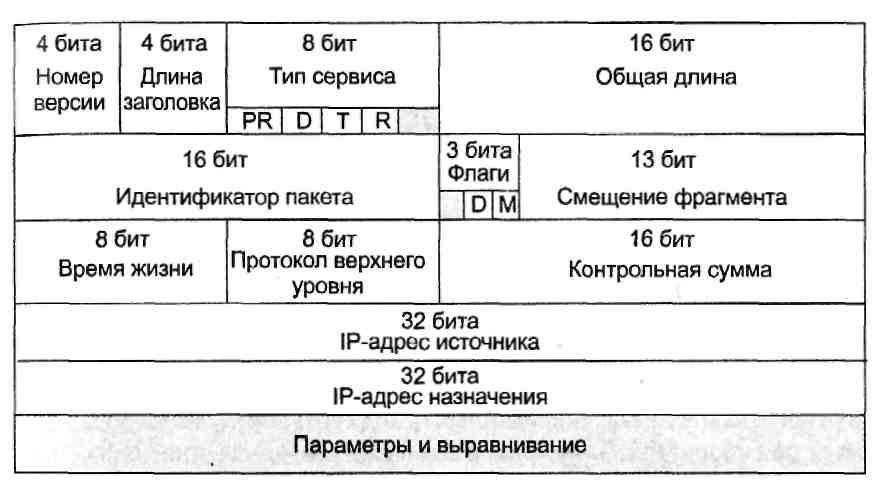
\includegraphics[width=0.9\textwidth]{photo/ipv4-header.jpg}
      \caption{Структура IPv4-заголовка}
      \label{ipv4-header}
    \end{figure}
      
    Обычно длина заголовка IP равна 20 байт, т.е. пять 32-битных слов, однако при увеличении объема служебной информации эта длина может быть увеличена
    за счет использования дополнительных байт в поле параметров и выравниваний. Благодаря полю, где содержится
    длина заголовка, можно правильно раскодировать оставшуюся последовательность байт. С помощью функций get\_ipv4\_data() и ipv4\_dec() будут получена 
    информация о времени жизни текущего пакета, о номере транспортного протокола, об IP-адресах отправителя и получателя.
  
    \begin{minted}[fontsize=\footnotesize]{Python}
      # Получение IPv4-заголовка
      def get_ipv4_data(data):
        version_header_length = data[0]
        header_length = (version_header_length & 15) * 4
        ttl, proto, src, dest = struct.unpack('!8xBB2x4s4s', data[:20])
        return ttl, proto, ipv4_dec(src), ipv4_dec(dest), data[header_length:]
      
      
      # Получение IP-адреса формата X.X.X.X
      def ipv4_dec(ip_bytes):
        ip_str = ''
        for el in ip_bytes:
          ip_str += str(el) + '.'
        return ip_str[:-1]
      
    \end{minted}

    После того, как был получен номер транспортного протокола, можно раскодировать их данные. Как уже упоминалось ранее, в качестве транспортных протоколов
    будут рассматриваться TCP и UDP протоколы. На рисунке \ref{tcp-header} изображена структура tcp-заголовка.
  
    \begin{figure}[H]
      \centering
      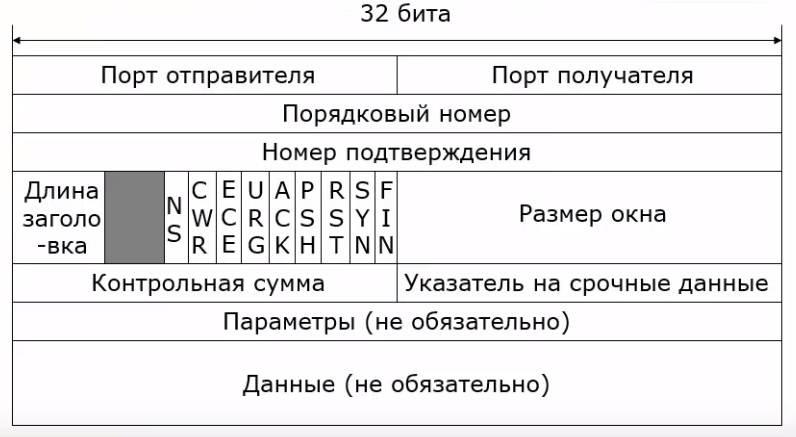
\includegraphics[width=0.9\textwidth]{photo/tcp-segment.jpg}
      \caption{Структура TCP-заголовка}
      \label{tcp-header}
    \end{figure}
    
    С помощью функции get\_tcp\_segment() производится получение информации, содержащейся в TCP-протоколе. Получается, теперь программе известны порт получателя,
    порт отправителя, порядковый номер, номер подтверждения и флаги. Однако самая ценная информация для данной работы --- это порты и данные, которые
    содержатся в TCP- и UDP-заголовках.

    \begin{minted}[fontsize=\footnotesize]{Python}
      # Получение TCP-cегмента данных
      def get_tcp_segment(data):
        src_port, dest_port, sequence, ack, some_block = struct.unpack('!HHLLH', data[:14])
        return src_port, dest_port, sequence, ack, data[(some_block >> 12) * 4:]
    
    \end{minted}

    Аналогично получается раскодирование данных UDP-заголовка с помощью функции get\_udp\_segment().

    \begin{minted}[fontsize=\footnotesize]{Python}
      # Получение UDP-сегмента данных
      def get_udp_segment(data):
        src_port, dest_port, size = struct.unpack('!HH2xH', data[:8])
        return src_port, dest_port, size, data[8:]
    \end{minted}      

    Далее необходимо рассмотреть данные, полученные после обработки TCP- и UDP-заголовков. В функции scan\_port() проверяется порт очередного пакета.
    Если порт совпадает с портом, заданным в начале программы (по умолчанию он равен 3389), то значит осуществляется попытка подключения к удаленному рабочему
    столу устройства, находящегося в текущей локальной сети. Также здесь осуществляется проверка известных IP-адресов, взятых из файла white-list.log. 

    \begin{minted}[fontsize=\footnotesize]{Python}
      # Проверка порта по-умолчанию
      def scan_port(src_ipv4, dest_ipv4, src_mac, src_port, dest_port):
        if dest_port == def_port:
          fl = False
          for key in white_list.keys():
            if key[1] == src_ipv4:
              fl = True
              break
          if not fl:
            for key in white_list.keys():
              if key[1] == dest_ipv4:
                tup = (src_ipv4, src_mac)    
                if tup not in black_list:
                  black_list.append(tup)
                  write_to_file((src_ipv4, src_mac, key[0], src_port, dest_port), False)
    \end{minted}

    В функции scan\_inf() производится анализ данных сегмента TCP, а \\* format\_data() --- функция для корректного представления полученных данных.

    \begin{minted}[fontsize=\footnotesize]{Python}
      # Проверка данных TCP-сегмента
      def scan_inf(r_data, src_ipv4, dest_ipv4, src_mac, dest_mac, dest_port, src_port):
        global Current_object
        global black_list
        global Packet_cnt
        data = format_data(r_data)
        flag = False
        for key in white_list.keys():
          if key[1] == src_ipv4:
            flag = True
            break
        if not flag:
          for key, value in white_list.items():
            if value[1] in data and key[1] == dest_ipv4:
              Current_object = (key[0], key[1], value[0])
              tup = (src_ipv4, src_mac)
              if tup not in black_list:
                  black_list.append(tup)
                  write_to_file(( src_ipv4, src_mac, Current_object[0]
                                , src_port, dest_port ), False)
          if Current_object:
            if Current_object[2] in data:
              for key in white_list.keys():
                if key[1] == src_ipv4:
                  write_to_file(( dest_ipv4, dest_mac, Current_object[0]
                                , src_port, dest_port ), True)
                  break
              Current_object = ''
            else:
              Packet_cnt += 1
              if Packet_cnt > 100:
                Packet_cnt = 0
                Current_object = '' 
    \end{minted}
    
    После вызова функции get\_tcp\_segment() могут быть получены данные, которые уже относятся к прикладному уровню. И такую последовательность чисел
    можно раскодировать IP-адрес и имя компьютера, показанных на рисунках \ref{clnt-hello} и \ref{serv-hello}.

    Практически все выше перечисленные функции содержатся в start\_to\_listen(), где производится вывод в консоль информации о получаемых пакетах, делаются
    вызовы функций для раскодирования последовательности чисел.

    \begin{minted}[fontsize=\footnotesize]{Python}

      # Перехват трафика и вывод информации в консоль
      def start_to_listen(interface):
        global Current_object
        global Cur_number
        os.system(f'ip link set {socket.if_indextoname(interface)} promisc on')
        server = socket.socket(socket.AF_PACKET, socket.SOCK_RAW, socket.ntohs(3))
        # server.bind((socket.if_indextoname(interface), 0))
        while True:
          # Получение пакетов в виде набора hex-чисел
          raw_data, _ = server.recvfrom(65565)
          dest_mac, src_mac, protocol = get_ethernet_frame(raw_data)
      
          # Если это интернет-протокол четвертой версии    
          if protocol == 8:
            print(f'-------------------Пакет N{Cur_number}-----------------------')
            Cur_number += 1
            print('Ethernet кадр: ')
            print('MAC-адрес отправителя: ' + str(src_mac), 'MAC-адрес получателя: ' + str(dest_mac))
            ttl, proto, src_ipv4, dest_ipv4, data_ipv4 = get_ipv4_data(raw_data[14:])
            print('IPv4 заголовок:')
            print( 'TTL: ' + str(ttl)
                 , 'Номер протокола: ' + str(proto)
                 , 'IP-адрес отправителя: ' + str(src_ipv4)
                 , 'IP-адрес получателя: ' + str(dest_ipv4))
            # Если это UDP-протокол  
            if proto == 17:
              src_port_udp, dest_port_udp, size, data_udp = get_udp_segment(data_ipv4)
              print('UDP заголовок:')
              print( 'Порт отправителя: ' + str(src_port_udp), 'Порт получателя: ' + 
                     str(dest_port_udp), 'Размер: ' + str(size) )
              
              scan_port(src_ipv4, dest_ipv4, src_mac, src_port_udp, dest_port_udp)
            # Если это TCP-протокол  
            if proto == 6:
              src_port_tcp, dest_port_tcp, sequence, ack, data_tcp = get_tcp_segment(data_ipv4)
              print('TCP заголовок:')
              print( 'Порт отправителя: ' + str(src_port_tcp)
                   , 'Порт получателя: ' + str(dest_port_tcp)
                   , 'Порядковый номер: ' + str(sequence)
                   , 'Номер подтверждения: ' + str(ack) )
      
              scan_port(src_ipv4, dest_ipv4, src_mac, src_port_tcp, dest_port_tcp)
              
              th_inf = threading.Thread(target=scan_inf, args=[ data_tcp
                                                              , src_ipv4
                                                              , dest_ipv4
                                                              , src_mac
                                                              , dest_mac
                                                              , dest_port_tcp
                                                              , src_port_tcp ])
              th_inf.start()
            keyboard.add_hotkey('Space', wait_key)
    \end{minted}

    После описания всех главных функций можно перейти к проверке корректности работы программы.

  \section{Демонстрация работы программы}
  Допустим к локальной сети подключено несколько устройств. Для тестирования данной программы было запущено четыре виртуальных машины:

  \begin{itemize}
    \item компьютер №1 с операционной системой Windows 10 Professional версии 21H2 IP-адресом 192.168.10.229
    \item компьютер №2 с операционной системой Windows 10 Professional версии 21H2 IP-адресом 192.168.10.254
    \item компьютер №3 с операционной системой Windows 10 Professional версии 21H2 IP-адресом 192.168.10.21
    \item компьютер №4 с операционной системой Linux Ubuntu версии 22.04 LTS IP-адресом 192.168.10.107
  \end{itemize}

  В ходе работы был создан файл white-list.log в который записаны имена компьютеров и их IP-адреса. Содержимое файла показано на
  рисунке \ref{white-list}.

  \begin{figure}[H]
    \centering
    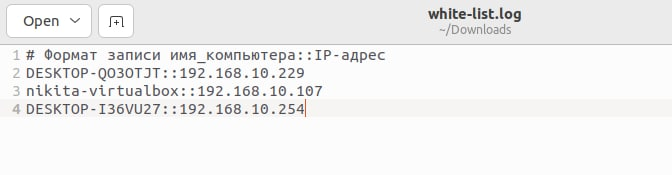
\includegraphics[width=0.9\textwidth]{photo/white-list.png}
    \caption{Содержимое файла white-list.log}
    \label{white-list}
  \end{figure}
  
  Стоит отметить, что информация о компьютере №3 не добавлена специально, так как его будут считать неизвестным устройством, остальные,
  информация о которых записана в файл, являются известными соответственно.
  
  Теперь необходимо провести несколько тестирований данной программы:

  \begin{enumerate}
    \item Пусть компьютер №3 выполнит подключение к компьютеру №1, где в это время на компьютере №4 будет уже работать программа rdp-sniffer.py.
    
    Из рисунка \ref{cmd-sniff1} видно, как программа запрашивает порт по умолчанию, а затем предоставляет выбор сетевого интерфейса. 

    \begin{figure}[H]
      \centering
      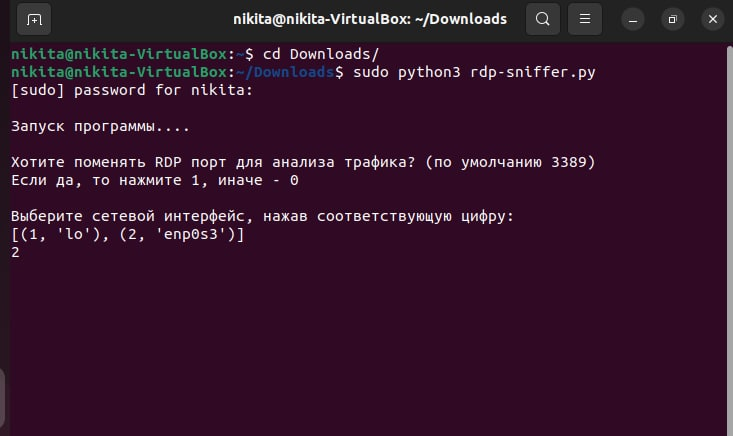
\includegraphics[width=0.9\textwidth]{photo/cmd-sniff1.png}
      \caption{Вид консоли при запуске программы}
      \label{cmd-sniff1}
    \end{figure}

    После осуществления подключения к удаленному рабочему столу в консоли начали появляться записи о пакетах, которые относятся к протоколу RDP, как показано на рисунке
    \ref{cmd-sniff2}.

    \begin{figure}[H]
      \centering
      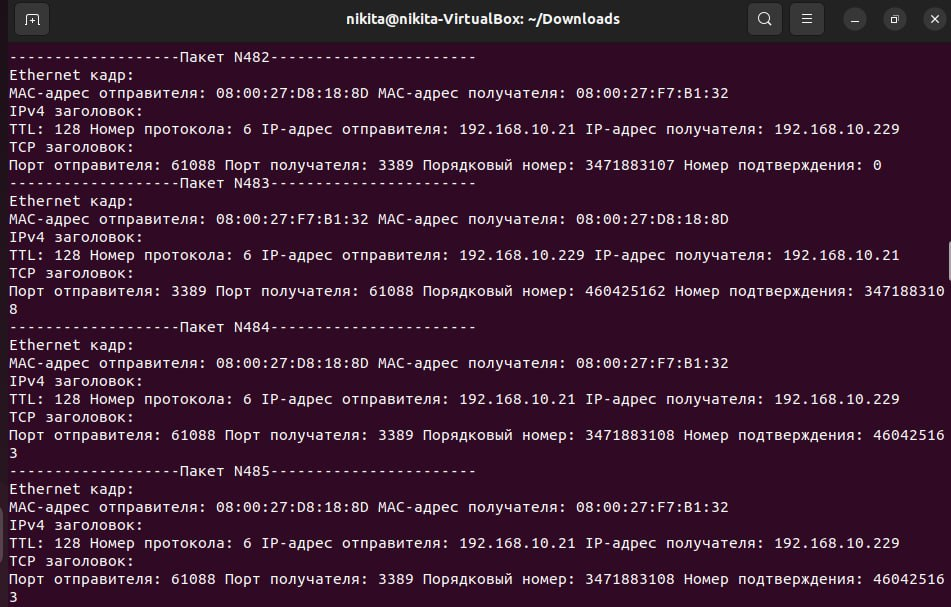
\includegraphics[width=0.9\textwidth]{photo/cmd-sniff2.png}
      \caption{Вид консоли при работе программы}
      \label{cmd-sniff2}
    \end{figure}

    Видно, что пакеты доставляются через TCP-порт 3389 протокола RDP. Теперь осталось проверить появились ли какие-нибудь записи в файле information.log.

    На рисунке \ref{inf-log1} изображены 3 записи, одна из которых была сделана из-за обнаружения 3389-го порта, а две записи --- при раскодировании данных протокола
    TLS. При анализе трафика с помощью программы Wireshark также наблюдались повторяющиеся пакеты протокола TLS, в которых содержалась практически одна и та же
    информация. Скорее всего это связано с тем, что устройства в процессе обмена данными <<договорились>> между собой, например, об изменении шифра или порта.
    Поэтому такого рода пакеты приходится отправлять повторно. Так как программа отслеживает
    все такие пакеты, то в файл было сделано две записи в разные моменты времени.

    \begin{figure}[H]
      \centering
      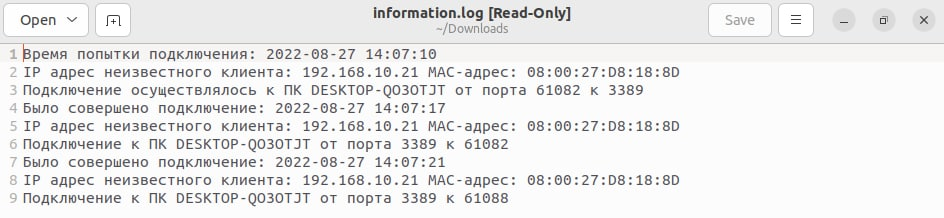
\includegraphics[width=0.9\textwidth]{photo/inf-log1.png}
      \caption{Содержимое файла information.log после подключения по порту 3389}
      \label{inf-log1}
    \end{figure}

    Таким образом благодаря файлу information.log можно узнать время установки RDP-сессии, IP-адрес и MAC-адрес неизвестного клиента

    \item Допустим будет совершено подключение по другому RDP порту или в программе ввести совсем другой порт, по которому будет проводится анализ пакетов.
    Пусть Компьютер №3 будет подключаться к компьютеру №1 по порту, например 13389, как показано на рисунке \ref{other-port}.

    \begin{figure}[H]
      \centering
      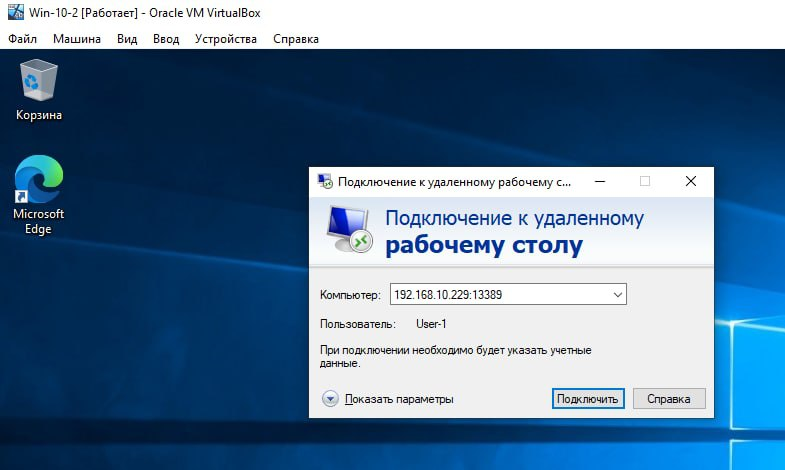
\includegraphics[width=0.9\textwidth]{photo/13389.png}
      \caption{Подключение к компьютеру №1 по другому порту}
      \label{other-port}
    \end{figure}

    Тогда при подключении к удаленному рабочему столу в файле \\* information.log появятся следующие записи, которые изображены на рисунке \ref{inf-log2}.

    \begin{figure}[H]
      \centering
      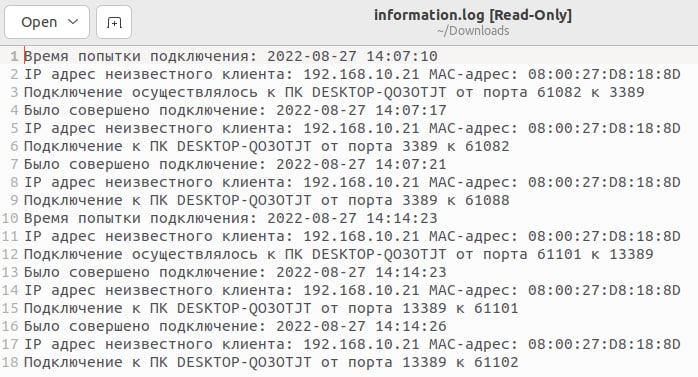
\includegraphics[width=0.9\textwidth]{photo/inf-log2.png}
      \caption{Содержимое файла information.log после подключения по порту 13389}
      \label{inf-log2}
    \end{figure}

    Получается программа установила то, что RDP-сессия произошла, опираясь на данные, которые содержатся в сообщениях протокола TLS.

    \item Теперь осталось проверить подключение по протоколу RDP компьютера №2 к компьютеру №1. При установки RDP-сессии программа отслеживает пакеты,
    как показано на рисунке \ref{cmd-sniff3}. 

    \begin{figure}[H]
      \centering
      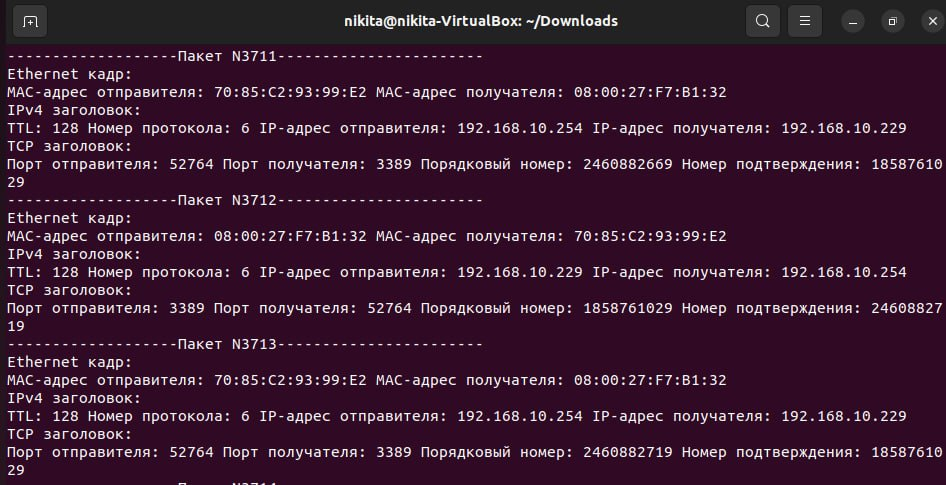
\includegraphics[width=0.9\textwidth]{photo/cmd-sniff3.png}
      \caption{Вид консоли при подключении к удаленному рабочему столу}
      \label{cmd-sniff3}
    \end{figure}

    Стоит отметить, что в файл information.log записи не были сделаны. Компьютер №2 считается
    верифицированным устройством, так как информация о нем содержится в файле white-list.log. Это сделано для того чтобы можно было точно определять
    несанкционированные подключения к удаленному рабочему столу.
  \end{enumerate}

  
  % Одним из таких методов обнаружения является клавиатурный мониторинг. Допустим может возникнуть ситуация, когда злоумышленник уже смог подключиться к
  % удаленному рабочему столу локального пользователя. Его сертификат оказался действительным, и он может полностью взять под свой контроль чужой компьютер.
  % И тогда у локального пользователя остается мало шансов предотвратить утечку информации.
  
  % И здесь одним из способов обнаружения RDP-сессии может быть полезен кейлоггер. Это программное обеспечение или аппаратное устройство, регистрирующее
  % различные действия пользователя — нажатия клавиш на клавиатуре компьютера, движения и нажатия клавиш мыши и т.д. \cite{keylog}. В данном случае кейлоггер
  % выполняет следующие задачи:
  
  % \begin{itemize}
  %   \item регистрирует нажатия клавиш на клавиатуре и мыши компьютера;
  %   \item при достижении заданного предела символов отправляет по протоколу SMTP (Simple Mail Transfer Protocol --- протокол передачи почты) сообщение на
  %   электронную почту;
  %   \item создает log-файл, в который делаются записи названия клавиш и их время удержания, а также названия клавиш мыши и их позиция на экране, представленная
  %   в виде двух координат.  
  % \end{itemize}

  % Чтобы обезопасить свой компьютер от сторонних подключений, локальный пользователь запускает программу кейлоггер, написанную на языке Python. Из рисунка \ref{cmd}
  % видно, что программа запрашивает логин и пароль от электронной почты, на которую будут отправляться сообщения.
  
  % \begin{figure}[H]
  %   \centering
  %   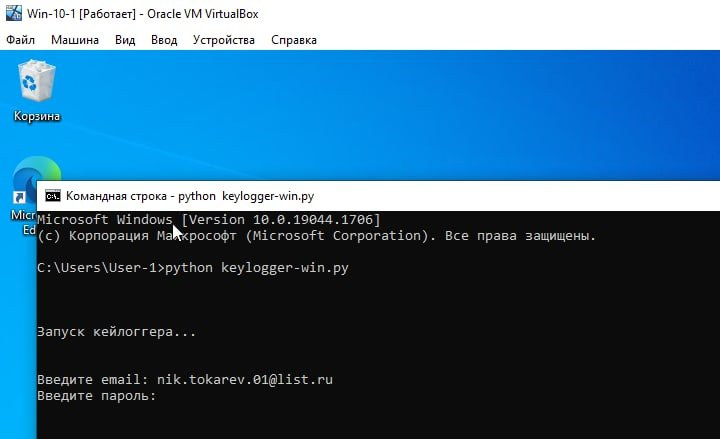
\includegraphics[width=0.9\textwidth]{photo/cmd.png}
  %   \caption{Окно программы при работе кейлоггера}
  %   \label{cmd}
  % \end{figure}

  % Допустим злоумышленник уже знает IP-адрес и имя пользователя компьютера, и ему удалось подключится к удаленному рабочему столу. На рисунке \ref{input1} показано
  % подключение к удаленному рабочему столу, а именно к компьютеру с IP-адресом 192.168.10.229. Стоит отметить, что здесь подключение производятся через
  % известное приложение для удаленного рабочего стола устройства Windows. Конечно, злоумышленник будет использовать программу, сигнатура которой никому другому
  % неизвестна. Поэтому программа <<Подключение к удаленному рабочему столу>> используется в качестве примера.

  % На рисунке \ref{input1} показан ввод различной информации при успешно установленной RDP-сессии.

  % \begin{figure}[H]
  %   \centering
  %   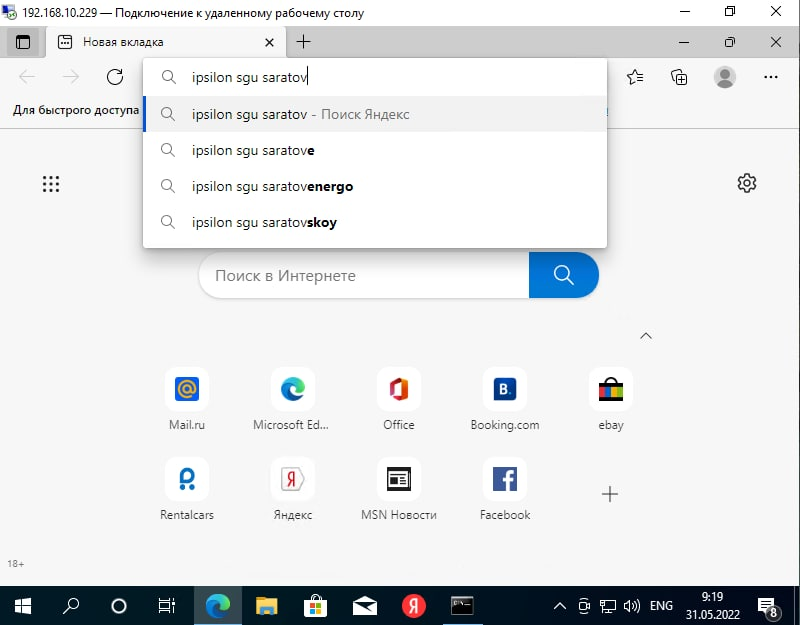
\includegraphics[width=0.9\textwidth]{photo/input1.png}
  %   \caption{Демонстрация работы с удаленным рабочим столом}
  %   \label{input1}
  % \end{figure}


  % Допустим злоумышленник решил попытаться зайти на сайт ipsilon.sgu.ru, зная логин и пароль некоторого пользователя, как показано на рисунке \ref{input2}.

  % \begin{figure}[H]
  %   \centering
  %   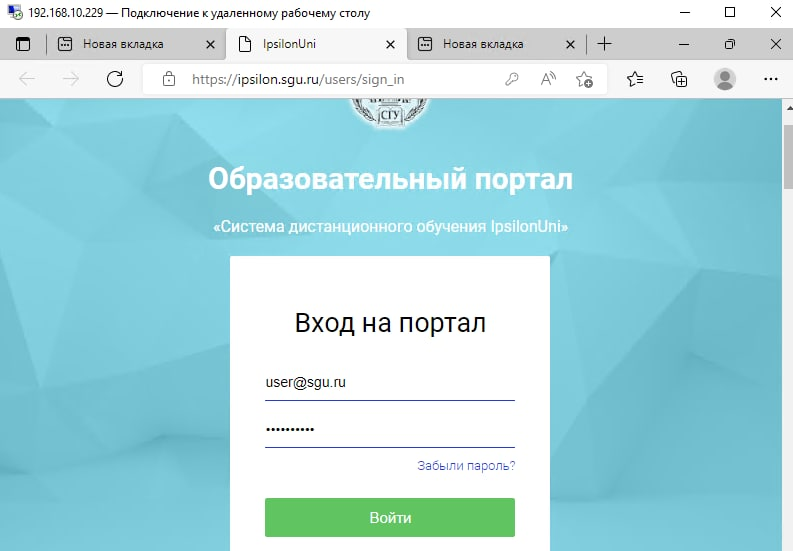
\includegraphics[width=0.9\textwidth]{photo/input2.png}
  %   \caption{Ввод логина и пароля, осуществляемый на сайте ipsilon.sgu.ru}
  %   \label{input2}
  % \end{figure}

  % И после набора определенного количества символов осуществляется отправка письма на электронную почту. На рисунке \ref{mailcheck} видно,
  % что письмо доставлено на введенную локальным пользователем почту.

  % \begin{figure}[H]
  %   \centering
  %   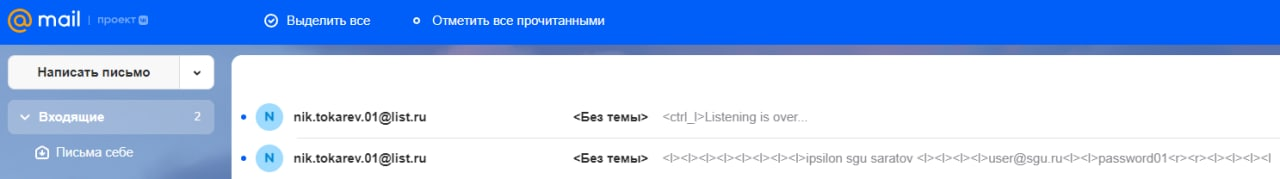
\includegraphics[width=0.9\textwidth]{photo/mail.png}
  %   \caption{Получение электронного письма}
  %   \label{mailcheck}
  % \end{figure}

  % На рисунке \ref{mail1} показано содержимое сообщения. Записи << <l> >> и << <r> >> обозначаются нажатия левой и правой кнопки мыши соответственно.

  % \begin{figure}[H]
  %   \centering
  %   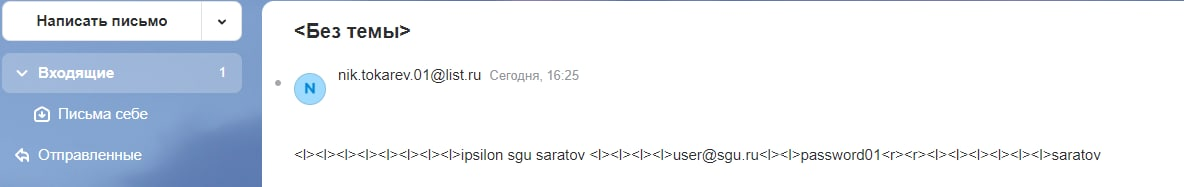
\includegraphics[width=0.9\textwidth]{photo/alsomail.png}
  %   \caption{Содержимое электронного письма}
  %   \label{mail1}
  % \end{figure}

  % Получив письмо, пользователь может начать действовать, пытаясь изолировать злоумышленника от интернета или просто зайдя под своей учетной записью на своем
  % устройстве. Таким образом RDP-сессия будет преддотвращена. При закрытии консоли или нажатии комбинации клавиш $Ctrl + f5$, программа завершает 
  % свою работу и в итоге получается log-файл, показанный на рисунке \ref{r1}. 
  
  
  % \begin{figure}[H]
  %   \centering
  %   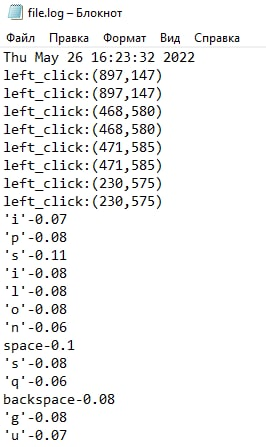
\includegraphics[width=0.4\textwidth]{photo/log-file.png}
  %   \caption{Содержимое файла file.log}
  %   \label{r1}
  % \end{figure}

  % Возможно ситуация, в которой злоумышленнику удается получить контроль над удаленным рабочим столом, маловероятна. Однако это не исключено. Ведь RDP блокирует
  % текущую сессию, где компьютер в данный момент работает, не позволяя двум пользователям видеть действия другого. В таком случае локальному пользователю будет сложно
  % остановить утечку данных, так как он не знает, когда была установлена RDP-сессия. Поэтому представленный в работе кейлоггер здесь может оказаться полезным.

  % \subsection{Другие варианты обнаружения RDP-сессии}

  % В Windows существуют логи RDP подключений, которые позволяют администраторам терминальных RDS серверов получить информацию о том, какие пользователи подключались
  % к серверу, когда сеанс был начат или завершен. Информация об этих событиях содержится в журналах Windows. Ее можно просмотреть, открыв коллекцию средств администрирования
  % --- <<Управление компьютером>>, позволяющая управлять локальным или удаленным компьютером. Открыв <<Просмотр событий>> необходимо рассмотреть следующее:

  % \begin{itemize}
  %   \item Network Connection ---  установка сетевого подключения к серверу от RDP клиента пользователя;
  %   \item Authentication --- успешная или неуспешная аутентификация пользователя на сервере;
  %   \item Session Disconnect/Reconnect --- события отключения/переподключения сессии имеют разные коды в зависимости от того, что вызвало отключение
  %   пользователя (отключение по неактивности, выбор пункта Disconnect в сессии, завершение RDP сессии другим пользователем или администратором и т.д.);
  %   \item Logon и Logoff --- RDP вход в систему и выход из системы. 
  % \end{itemize}

  % В перечисленных событиях необходимо анализировать значения EventID. Благодаря им, можно узнать некоторую информацию о возможных подключениях.
  % В основном просмотр логов RDP подключений осуществляется уже после того, как произошла какая-либо утечка информации. Благодаря просмотру событий
  % пользователь может предотвратить будущие атаки злоумышленников, однако он уже не сможет вернуть похищенные данные, которые производились в результате
  % установки посторонних RDP-сессий.

  \conclusion
  
  В результате проделанной работы были разобраны методы обнаружения подключения к удаленному рабочему столу по протоколу RDP, где с помощью различных программ
  удалось рассмотреть принцип работы RDP-протокола. Стоит отметить, что RDP далеко не самый защищенный протокол. Хотя корпорация Microsoft регулярно
  выпускает обновления для своего программного обеспечения. Однако RDP-сессия становится уязвимой из-за упущений в безопасности, например из-за
  некорректной конфигурации сервисов или установки устаревших обновлений системы. В таком случае злоумышленник может использовать такие просчеты в своих целях.
  А людям, ответственным за безопасность компьютерной сети, остается только придумывать новые методы обнаружения и предотвращения несанкционированных подключений
  к удаленному рабочему столу.


  \begin{thebibliography}{15}
    \bibitem{1}
    Книга Ибе О.С. «Компьютерные сети и службы удаленного доступа» / пер. с англ. -
    Москва, издательство: «ДМК Пресс», Яз. рус.
    \bibitem{2}
    Удалённый рабочий стол RDP: как включить и как подключиться по RDP [Электронный ресурс] / URL:https://hackware.ru/?p=11835 (дата обращения 03.05.2022), Яз. рус.
    \bibitem{userdp1}
    How to use remote desktop [Электронный ресурс] / URL: https://support.microsoft.com/en-us/windows/how-to-use-remote-desktop-5fe128d5-8fb1-7a23-3b8a-41e636865e8c (дата обращения 27.05.2022), Яз. англ.
    \bibitem{userdp2}
    Статья <<Как исправить ошибку удаленного рабочего стола не удается подключиться к удаленному компьютеру>> [Электронный ресурс] / URL: https://okdk.ru/kak-ispravit-oshibku-udalennogo-rabochego-stola-ne-udaetsya-podkljuchitsya-k-udalennomu-kompjuteru/ 
    (дата обращения 27.05.2022), Яз. рус.
    \bibitem{rdp2}
    Документация Remote Utilities <<RDP>> [Электронный ресурс] / URL:  https://www.remoteutilities.com/support/docs/rdp/ (дата обращения 27.05.2022), Яз. англ.
    % \bibitem{3}
    % Документация по устранению неполадок служб удаленных рабочих стола для Windows Server [Электронный ресурс] / URL: https://inlnk.ru/bvOV0 (дата обращения 04.05. 2022), Яз. рус.
    \bibitem{socket1}
    Документация по стандартным библиотекам языка Python [Электронный ресурс] / URL: https://docs.python.org/3/library/socket.html (дата обращения 25.06.2022), Яз. англ.
    \bibitem{socket2}
    Статья <<Интерактивная система просмотра системных руководств (man-ов)>> [Электронный ресурс] / URL: https://www.opennet.ru/cgi-bin/opennet/man.cgi?topic=socket\&category=2 (дата обращения 25.06.2022), Яз. англ.
    \bibitem{rdpudp}
    Документация Microsoft <<Протоколы>> [Электронный ресурс] / URL: https://docs.microsoft.com/en-us/openspecs/windows_protocols/ms-rdpeudp2/d8bf9a56-90f3-4608-8f98-9600ed69876b (дата обращения 28.05.2022), Яз. рус.
    \bibitem{rdp1}
    Статья <<Wireshark Tutorial: Decrypting RDP Traffic>> [Электронный ресурс] / URL: https://unit42-paloaltonetworks-com.translate.goog/wireshark-tutorial-decrypting-rdp-traffic/?_x_tr_sl=en\&_x_tr_tl=ru\&_x_tr_hl=ru\&_x_tr_pto=op,wapp
    (дата обращения 28.05.2022), Яз. англ.

  \end{thebibliography}

  \appendix

    \section{Код rdp-sniffer.py}
    \inputminted[fontsize=\footnotesize]{Python}{code/rdp-sniffer.py}

\end{document}